\documentclass[12pt]{article}
\title{\vspace{-1em}ML HW\#4}
\author{\vspace{-2em}Wei-Rou Lin, R05922128}
\date{}
\usepackage{indentfirst}
\usepackage[a4paper, vmargin=4em, hmargin=4em]{geometry}
\usepackage{amsmath} \usepackage{commath}
\usepackage{minted} \usepackage{xcolor}
\usepackage{graphicx}
\usepackage{listings} \usepackage{verbatimbox}
\usepackage{tabularx}
\setlength{\parindent}{2em}
\begin{document}
\tolerance=3000
\twocolumn
\setlength{\columnsep}{2em}
\maketitle
\section{Feature extraction}
  \par The bag-of-word model is used to extract the
  feature of the sentences. The terms are decided
  after stopword removal, stemming analysis and
  discarding the terms of which document frequency
  larger than 1/20 amount of the document set or
  smaller than 2. These processes result in 3588 terms.
  \par TF-IDF method is then taken to generate the sparse
  document-term matrix. After all of the above processes,
  two different decomposition methods are applied.
  Finally, the decomposed vectors are normalized for
  better clustering.
  \subsection{Decomposition Methods}
    \subsubsection{LSA}
    \par LSA is used to decompose the sparse
    document-term matrix. Fixing the cluster number
    to 20, I select an output dimension of 100 by
    minimize the coefficient of variation calculated
    on the cluster size.
    \subsubsection{Autoencoder}
    \par The autoencoder is a three-layered NN activated
    by sigmoid function. 20\% of the datas are splitted for
    validation. Binary-cross-entropy is chosen to be
    the loss function, and NADAM is applied to minimize the loss.
    \par To avoid overfitting, the validation loss is
    monitored during the training, which would be
    stopped after 30 epochs with no improvement.
    The best weigts of the NN leading to a minimum
    validation loss during the training is saved.
    \par Finally, the training stopped after 81 epochs.
    The minimum validation loss is 2.129e-3 and the
    training data loss at the same epoch is 1.248e-3.
    \subsection{Discussion}
    \par The Kaggle score of each decomposition methods
    are presented in Table \ref{score}. The score of
    autoencoder method is significantly higher than
    that of the LSA method with the same cluster number.
    This implies the autoencoder learned better
    semantic informations than LSA for the purpose of
    reconstrcuting the bag-of-word vectors.
    \par I've tried another method to decide whether or
    not the two given titles are in the same category
    without K-means clustering. The method is to search
    the titles with BM25F scoring using or group of
    terms in a title as a query. And then the first
    10000 results are taken as being in the same
    cluster as the query. The result is as well shown
    in Table \ref{score}, which is not satisfactory
    but expectable because of using a sparse vector to
    cluster the data directly without a decomposition
    method to extract the requisite sematic information
    in the sentences and without an advanced algorithm
    for clustering.
    \par Also, as I trying out different cluster numbers,
    the minimization of coefficient of variance
    calculated on cluster size becomes nonsense.
    Thus, I tuned the dimensions of decomposed
    vectors, but the difference of resulting score
    seems not as notable as changing the method
    or cluster number.
\begin{table}
  \centering
  \noindent
  \begin{tabular}{ccc}
    Feature & Cluster\# & Score\\
    \hline \space
    Autoencoder & 20 & 0.67149 \\
    LSA-100 & 20 & 0.48543 \\
    LSA-100 & 40 & 0.56591 \\
    LSA-100 & 100 & 0.37335 \\
    LSA-200 & 40 & 0.50552 \\
    BM25F & - & 0.41666 \\
    \hline \space
  \end{tabular}
  \caption{The resulting Kaggle score of different
  feature extraction and clustering implementations.}
  \label{score}
\end{table}
\section{Cluster numbers}
\par Drastic different results is provided by different
cluster numbers using K-means clustering. The
cluster\#-score relation is plotted in Figure \ref{cluster}.
The highest score is presented as setting the cluster
number to 40, two times as large as the real cluster number.
\par The K-means clustering will result in totally
different output each time even if we provide the
same input data, so the highest score at 40 cluster
number may just be a lucky try. However, Figure
\ref{cluster} still shows a tendency of accuracy as
the cluster number increased.
\begin{figure}
  \centering
  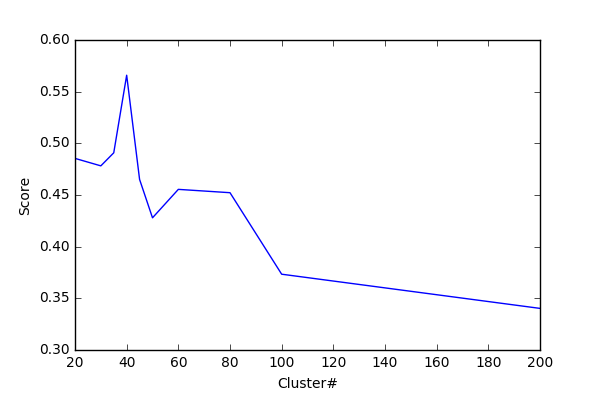
\includegraphics[width=0.75\linewidth]{cluster-score.png}
  \caption{The cluster\#-score plot with LSA-100,
  with cluster\# 20, 30, 35, 40,
  45, 50, 60, 80, 100 and 200, some scores of which are
  shown in Table \ref{score}.}
  \label{cluster}
\end{figure}
\section{Cluster word analysis}
\par Let's first define the "keyterm" of a cluster
as the term maximize the sum of the TF-IDF for all
sentences in the cluster. Then the keyterms of each
clustering experiment are shown in Table \ref{keyterm}.
\par Each keyterm extracted from true labels can be matched
one of the given tags, with the differences mostly come
from the stemming process. The only one match of
different terms even after stemming is osx/mac. Surprisingly,
the keyterms extracted from autoencoder clusters and from true
label clusters are {\bf exactly} the same.
\par In LSA-20, 3 terms are replaced to other terms,
two of which (it, what) seems not to provide information
in that cluster. I wondered if other terms
producing relatively large summation would provide a better
representation of the cluster, but neither are the top-5
terms of the two clusters (it, when, why, typ, doe; what,
way, best, ar, doe) more informative.
\par As the cluster number becoming larger in LSA-40, the
keyterms include all of those extracted in the true label
clusters. The extra terms are colored in Table \ref{keyterm}.
The sentences in the clusters with matched keyterms
are counted to 11755, which is a relatively large part
of the data.

\begin{table*}
  \label{keyterm}
  \noindent
  \newcommand{\diff}[1]{{\color{teal}#1}}
  \newcommand{\diffa}[1]{{\color{brown}#1}}
  \begin{tabular}{cm{0.75\textwidth}}
    Feature & Keyterms \\
    \hline \hline
    True Label &
    ajax, \diffa{apach}, bash, coco, drup, excel, haskel, hibern,
    linq, \diffa{mac}, magento, matlab, orac, qt, scal, sharepoint,
    \diffa{spring}, svn, vis, wordpress\\
    \hline
    Autoencoder&
    ajax, apach, bash, coco, drup, excel, haskel, hibern,
    linq, mac, magento, matlab, orac, qt, scal, sharepoint,
    spring, svn, vis, wordpress\\
    \hline
    LSA-20&
    ajax, bash, coco, drup, excel, haskel, hibern, \diff{it},
    linq, magento, matlab, orac, qt, scal, sharepoint,
    \diff{subvert}, svn, vis, \diff{what}, wordpress\\
    \hline
    LSA-40&
    ajax, \diff{ap}, apach, bash, coco,
    \diff{command}, \diff{cre}, \diff{custom}, \diff{dat},
    \diff{diff}, \diff{direct}, drup, \diff{er}, excel,
    \diff{get}, haskel, hibern, \diff{it}, linq, mac,
    magento, matlab, \diff{multipl}, \diff{net}, \diff{not},
    \diff{or}, orac, qt, scal, \diff{set}, sharepoint,
    spring, \diff{subvert}, svn, \diff{url}, vis, \diff{what},
    \diff{when}, wordpress, \diff{work}\\
    \space
    \hline \hline
    Tags &
    ajax, apache, bash, cocoa, drupal, excel, haskell, hibernate,
    linq, magento, matlab, oracle, osx, qt, scala, sharepoint,
    spring, svn, visual-studio, wordpress\\
    \hline
  \end{tabular}
  \caption{The keyterms extracted from different features.
  \diff{Teal} colored terms are terms not found on the
  clusters of true label, whereas \diffa{brown} colored
  terms are terms found on true label but not found on LSA-20.}
\end{table*}

\section{Visualization}
  \par To visualize the clustering results, PCA decomposition
  is applied to the sparse TF-IDF vectors, resulting in
  2-dimensional vectors which then taken to plot on Figure \ref{2dplot}.
  There seems to be three "branches" and a "core," and each
  method can easily distinguish the branches, but the difference
  in each results could lay in the core.
  \par We can take a closer look at the core via Figure \ref{center}.
  The centers of each cluster are scattered in the figure.
  "Explicit" terms such as {\bf matlab}, {\bf excel} are
  relatively close on the plane, and the feature resulting
  in better accuracy are closer to the true label generally.

\begin{figure}
  \centering
  \newcommand{\ww}{0.48}
  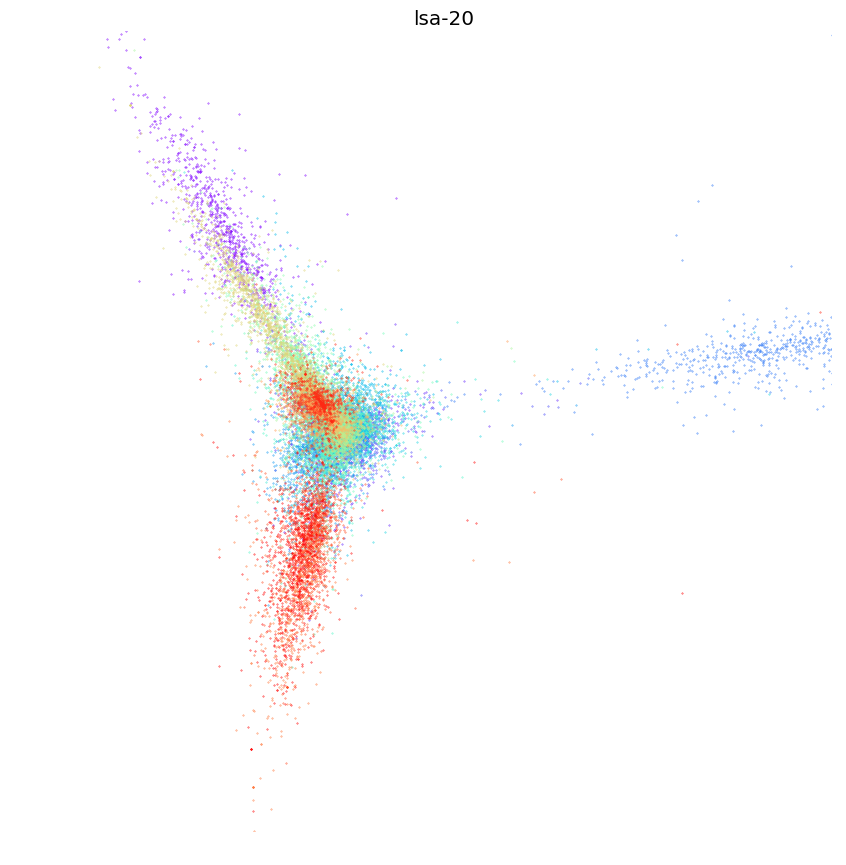
\includegraphics[width=\ww\linewidth]{lsa-20.png}
  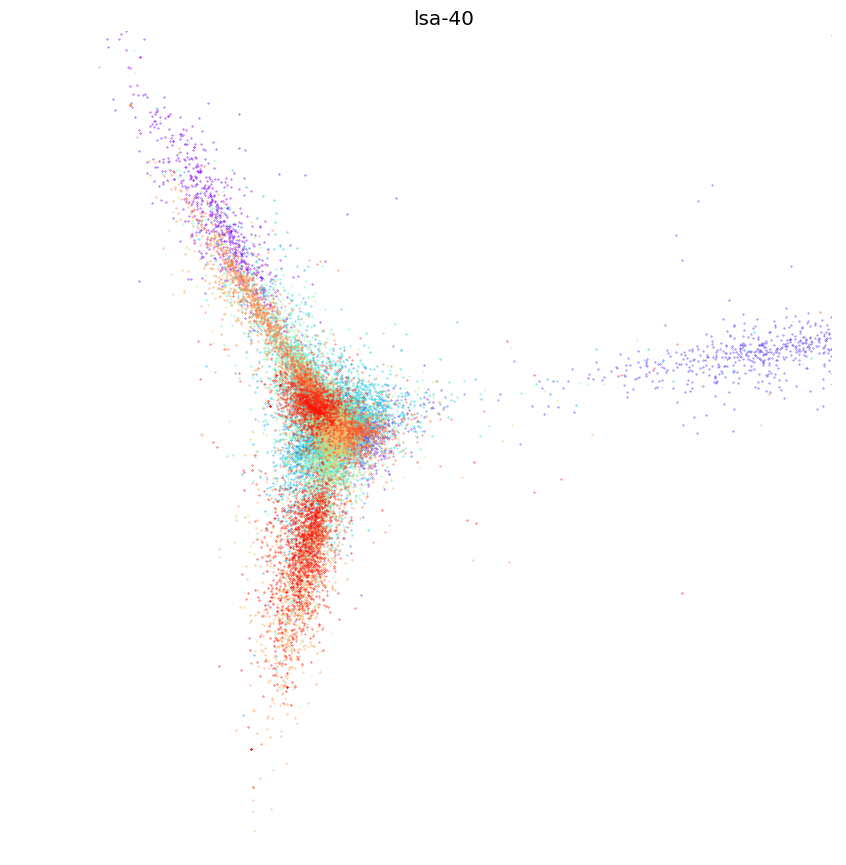
\includegraphics[width=\ww\linewidth]{lsa-40.png}
  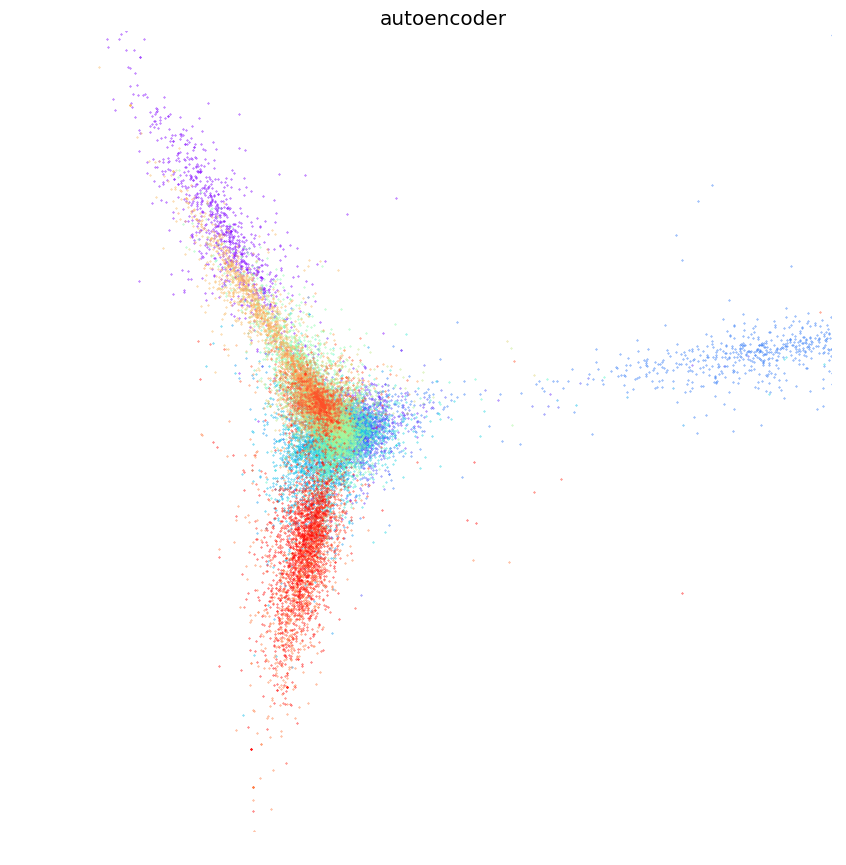
\includegraphics[width=\ww\linewidth]{autoencoder.png}
  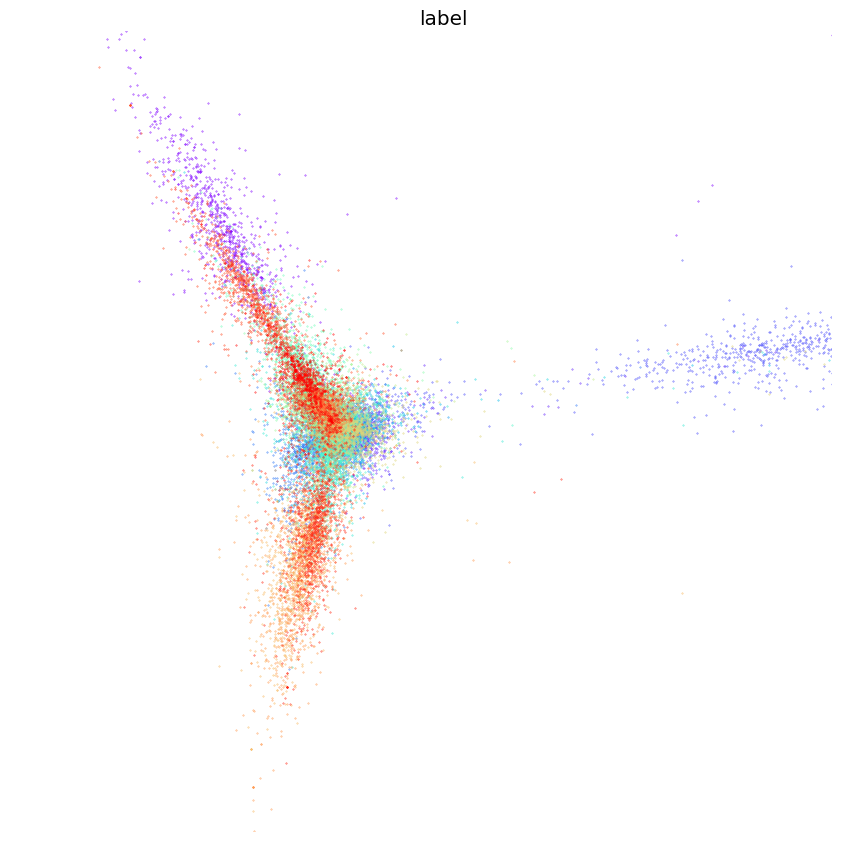
\includegraphics[width=\ww\linewidth]{label.png}
  \caption{The 2D decomposition of Sentence Vectors
  colored by clusters. The implementations from left
  to right, from top to bottom are LSA-20cluseters,
  LSA-40clusters and autoencoder-20clusters in turn,
  and the rightmost bottom one plots the true labels
  of the vectors.}
  \label{2dplot}
\end{figure}

\begin{figure*}
  \centering
  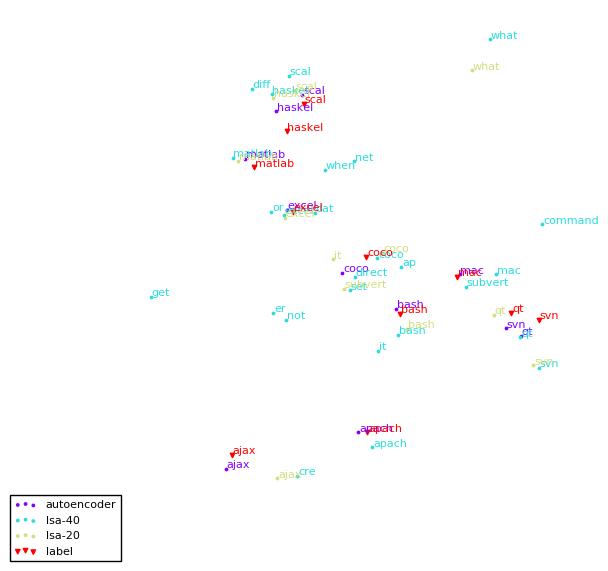
\includegraphics[width=0.9\linewidth]{centers.png}
  \label{center}
  \caption{The centers of each label colored by clustering
  results and marked by its keyterm. The "label" in the
  legend represent the true label of the data.}
\end{figure*}
\end{document}
